\pagestyle{fancy}

\graphicspath{ {Figures/Chapter4_ThermalModel/} }

The bulk of this thesis consisted in implementing a thermal simulation code able to reproduce the thermal evolution of thin target detectors during operation.
The program implemented by M. Sapinski in 2012 for fast wire scanner simulations \parencite[][]{ref:Msapinski} was taken as a starting point. The idea started by M. Sapinski, for fast wire scanner simulations, has been generalized to other types of thin target detectors, such as SEM grids, slow wire scanners and foils. 

\section{Introduction and Motivation}
\label{sec:Motivation}

During operation, interceptive devices interact directly with the beam of particles. As was discussed in chapter \ref{ch:BeamMatterInter}, the beam of particles deposits some energy in the detector's material. How much energy is deposited depends on the beam energy, the type of particle but also material detector and geometry. This deposited energy leads to a fast increase of the detector temperature. Depending on the beam conditions, the thermal shock suffered by the detectors can be very severe. This might affect the measured currents (Thermionic Emission), or in some cases permanently manage the detectors. 

\begin{figure}[h]
    \centering
    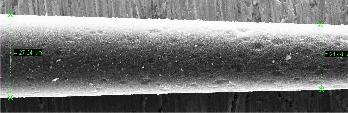
\includegraphics[width=0.60\columnwidth]{WireRadiusDeterioration/WireDamage.png}
    \caption{Carbon fiber wire scanner used at SPS in 2008.}
    \label{fig:WireRadius}
\end{figure}

Figure \ref{fig:WireRadius} shows a picture of a wire scanner photographed with a scanning electron microscope. This scanner was used in 2008 at CERN SPS during a systematic breakage experiment \parencite[][]{ref:Msapinski}. This picture shows how the radius of the wire was reduced due to the sublimation process after consecutively reaching high temperatures.

Another clear example of detector damage due to high temperature can be observed in Figure \ref{fig:SEMLinac4damage}. In this case, we can observe three pictures taken from a SEM grid used at LINAC4 in 2019. This grid had 40 $\mu m$ gold-coated tungsten wires. Already in the first picture (left) one can observe how the gold coating was evaporated from the wires in the central part of the grid (Gold Melting Temperature is ~ 1400 K). From the images taken with the optical microscope (right), we can observe two wires glued together due to the high temperatures reached by the detector. To avoid these permanent damages, a deep understanding of the thermal evolution suffered by the detectors is necessary. 
\begin{figure}[h]
    \centering
    \begin{subfigure}[b]{0.42\textwidth}
        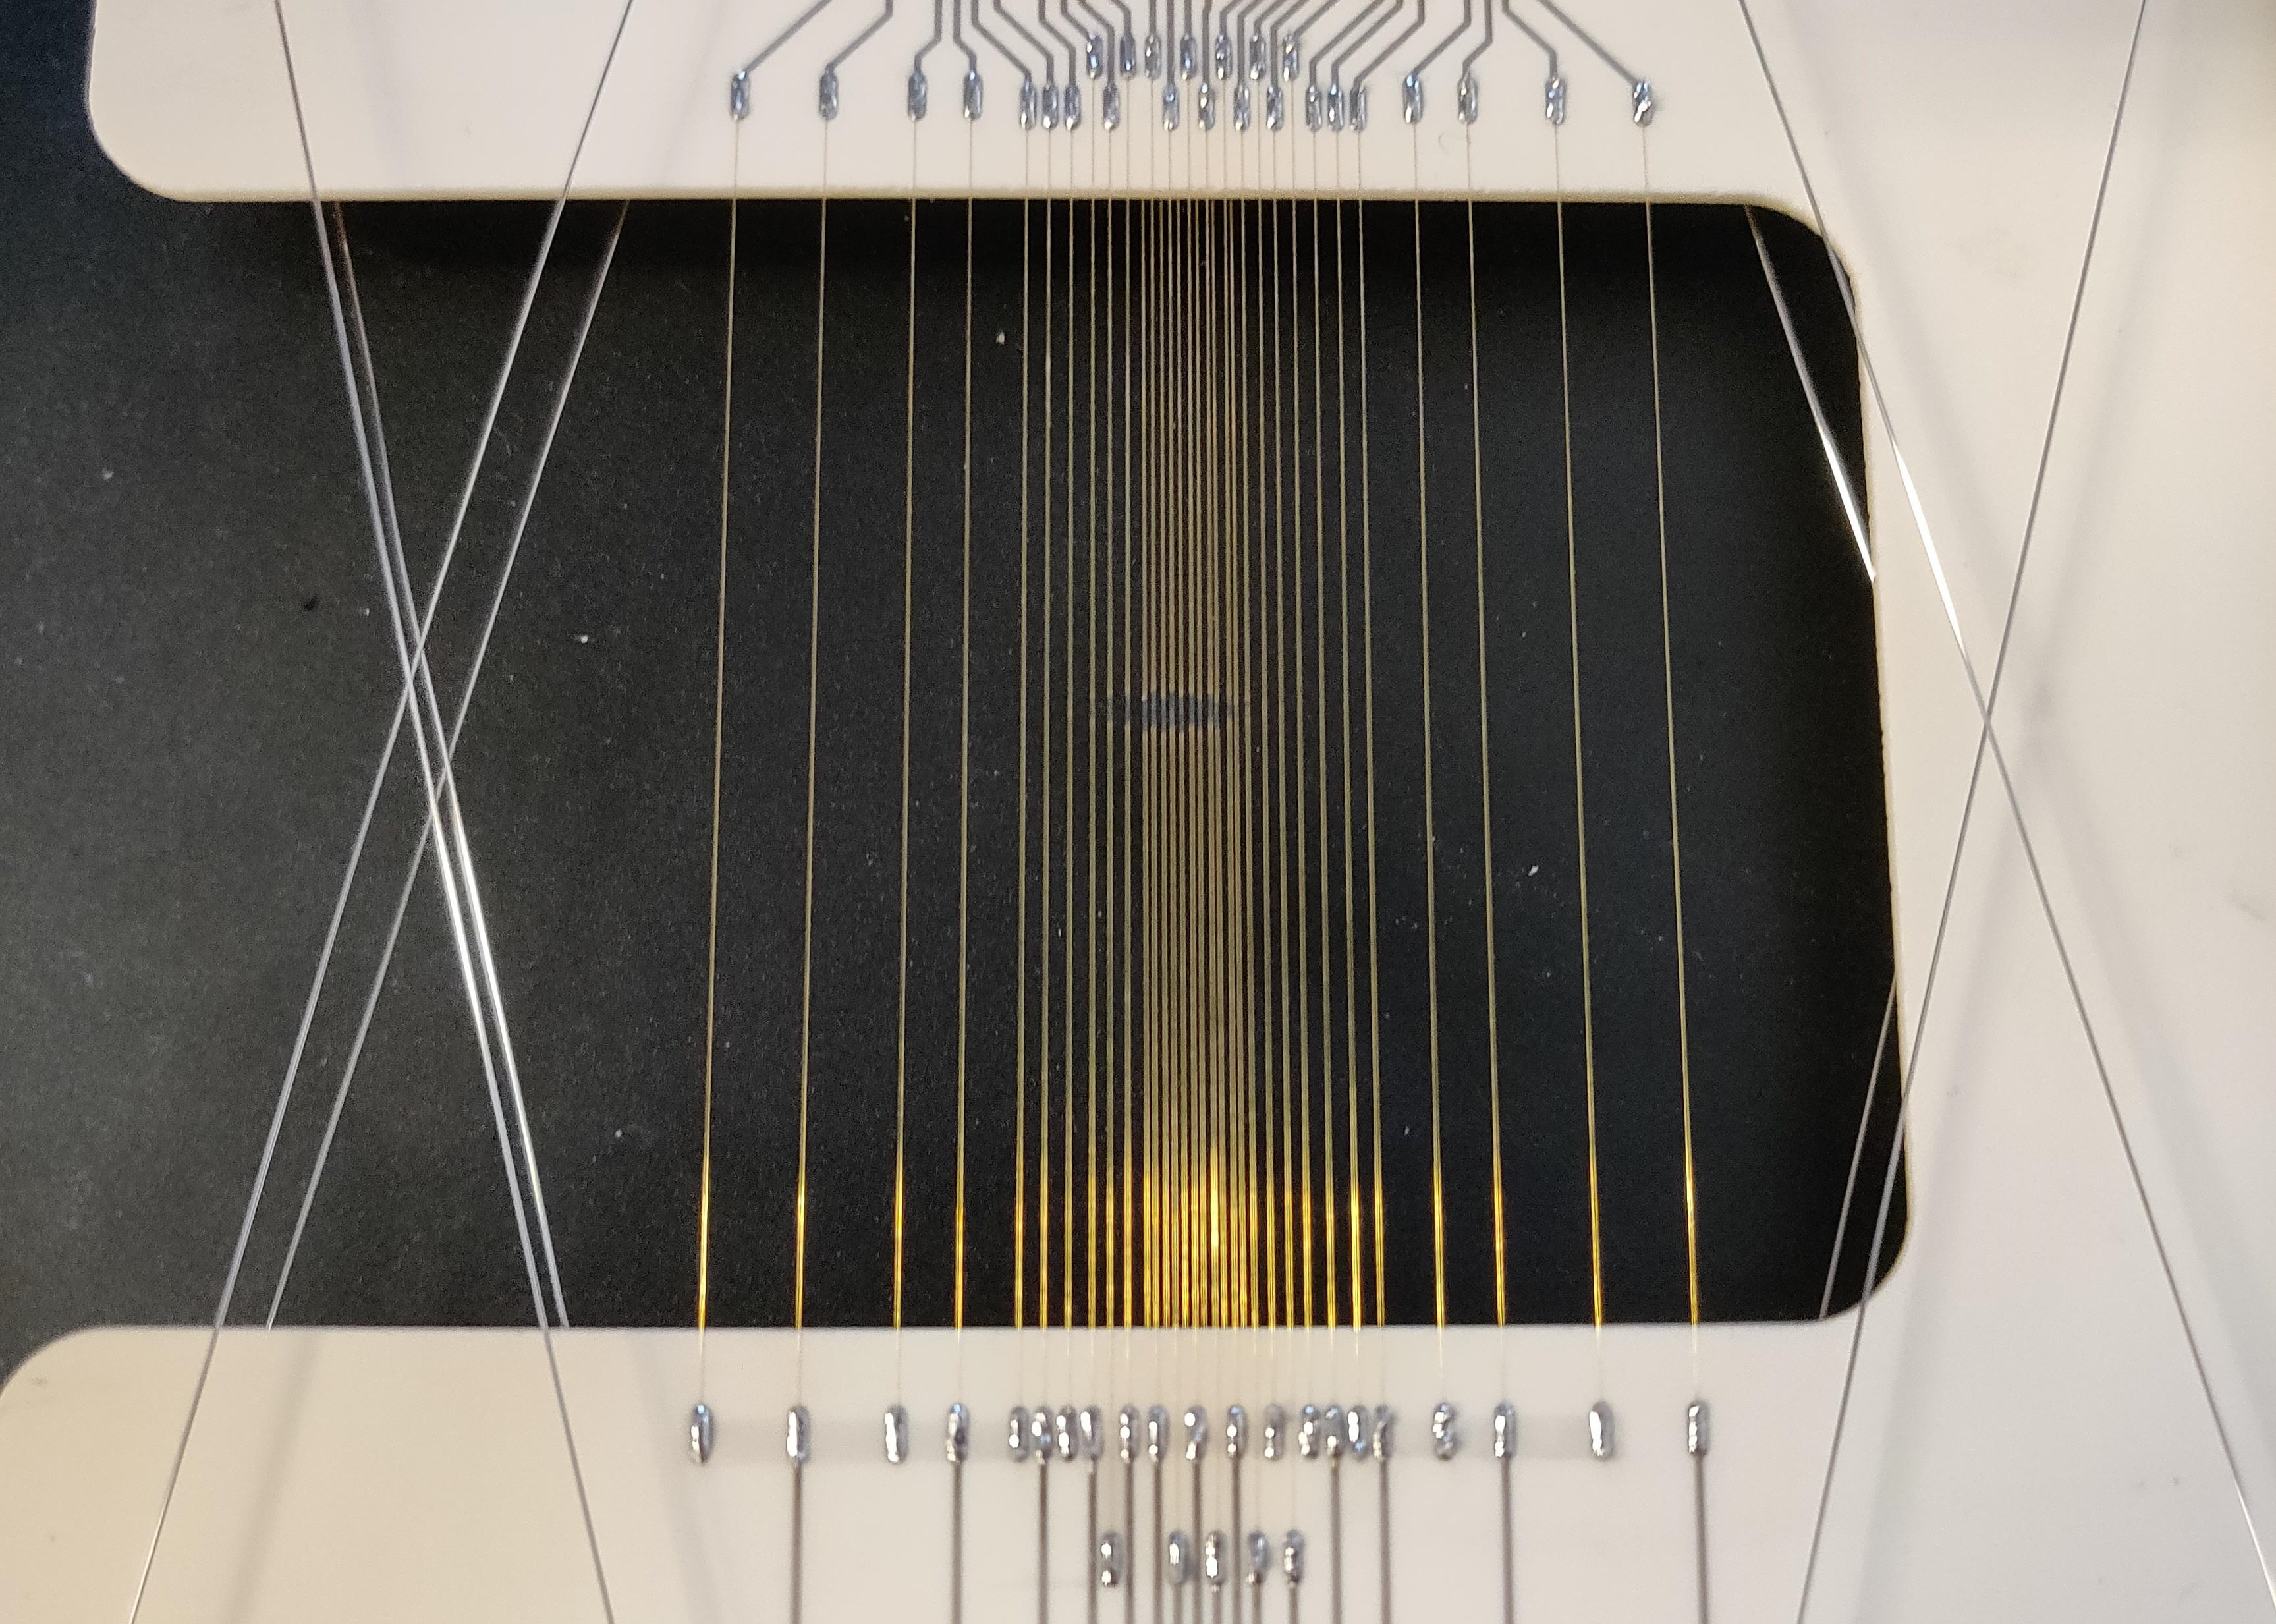
\includegraphics[width=\textwidth]{SEMgridDamage/GridDamage1.jpg}
    \end{subfigure}
    \hspace{0.5cm}
    \begin{subfigure}[b]{0.4\textwidth}
        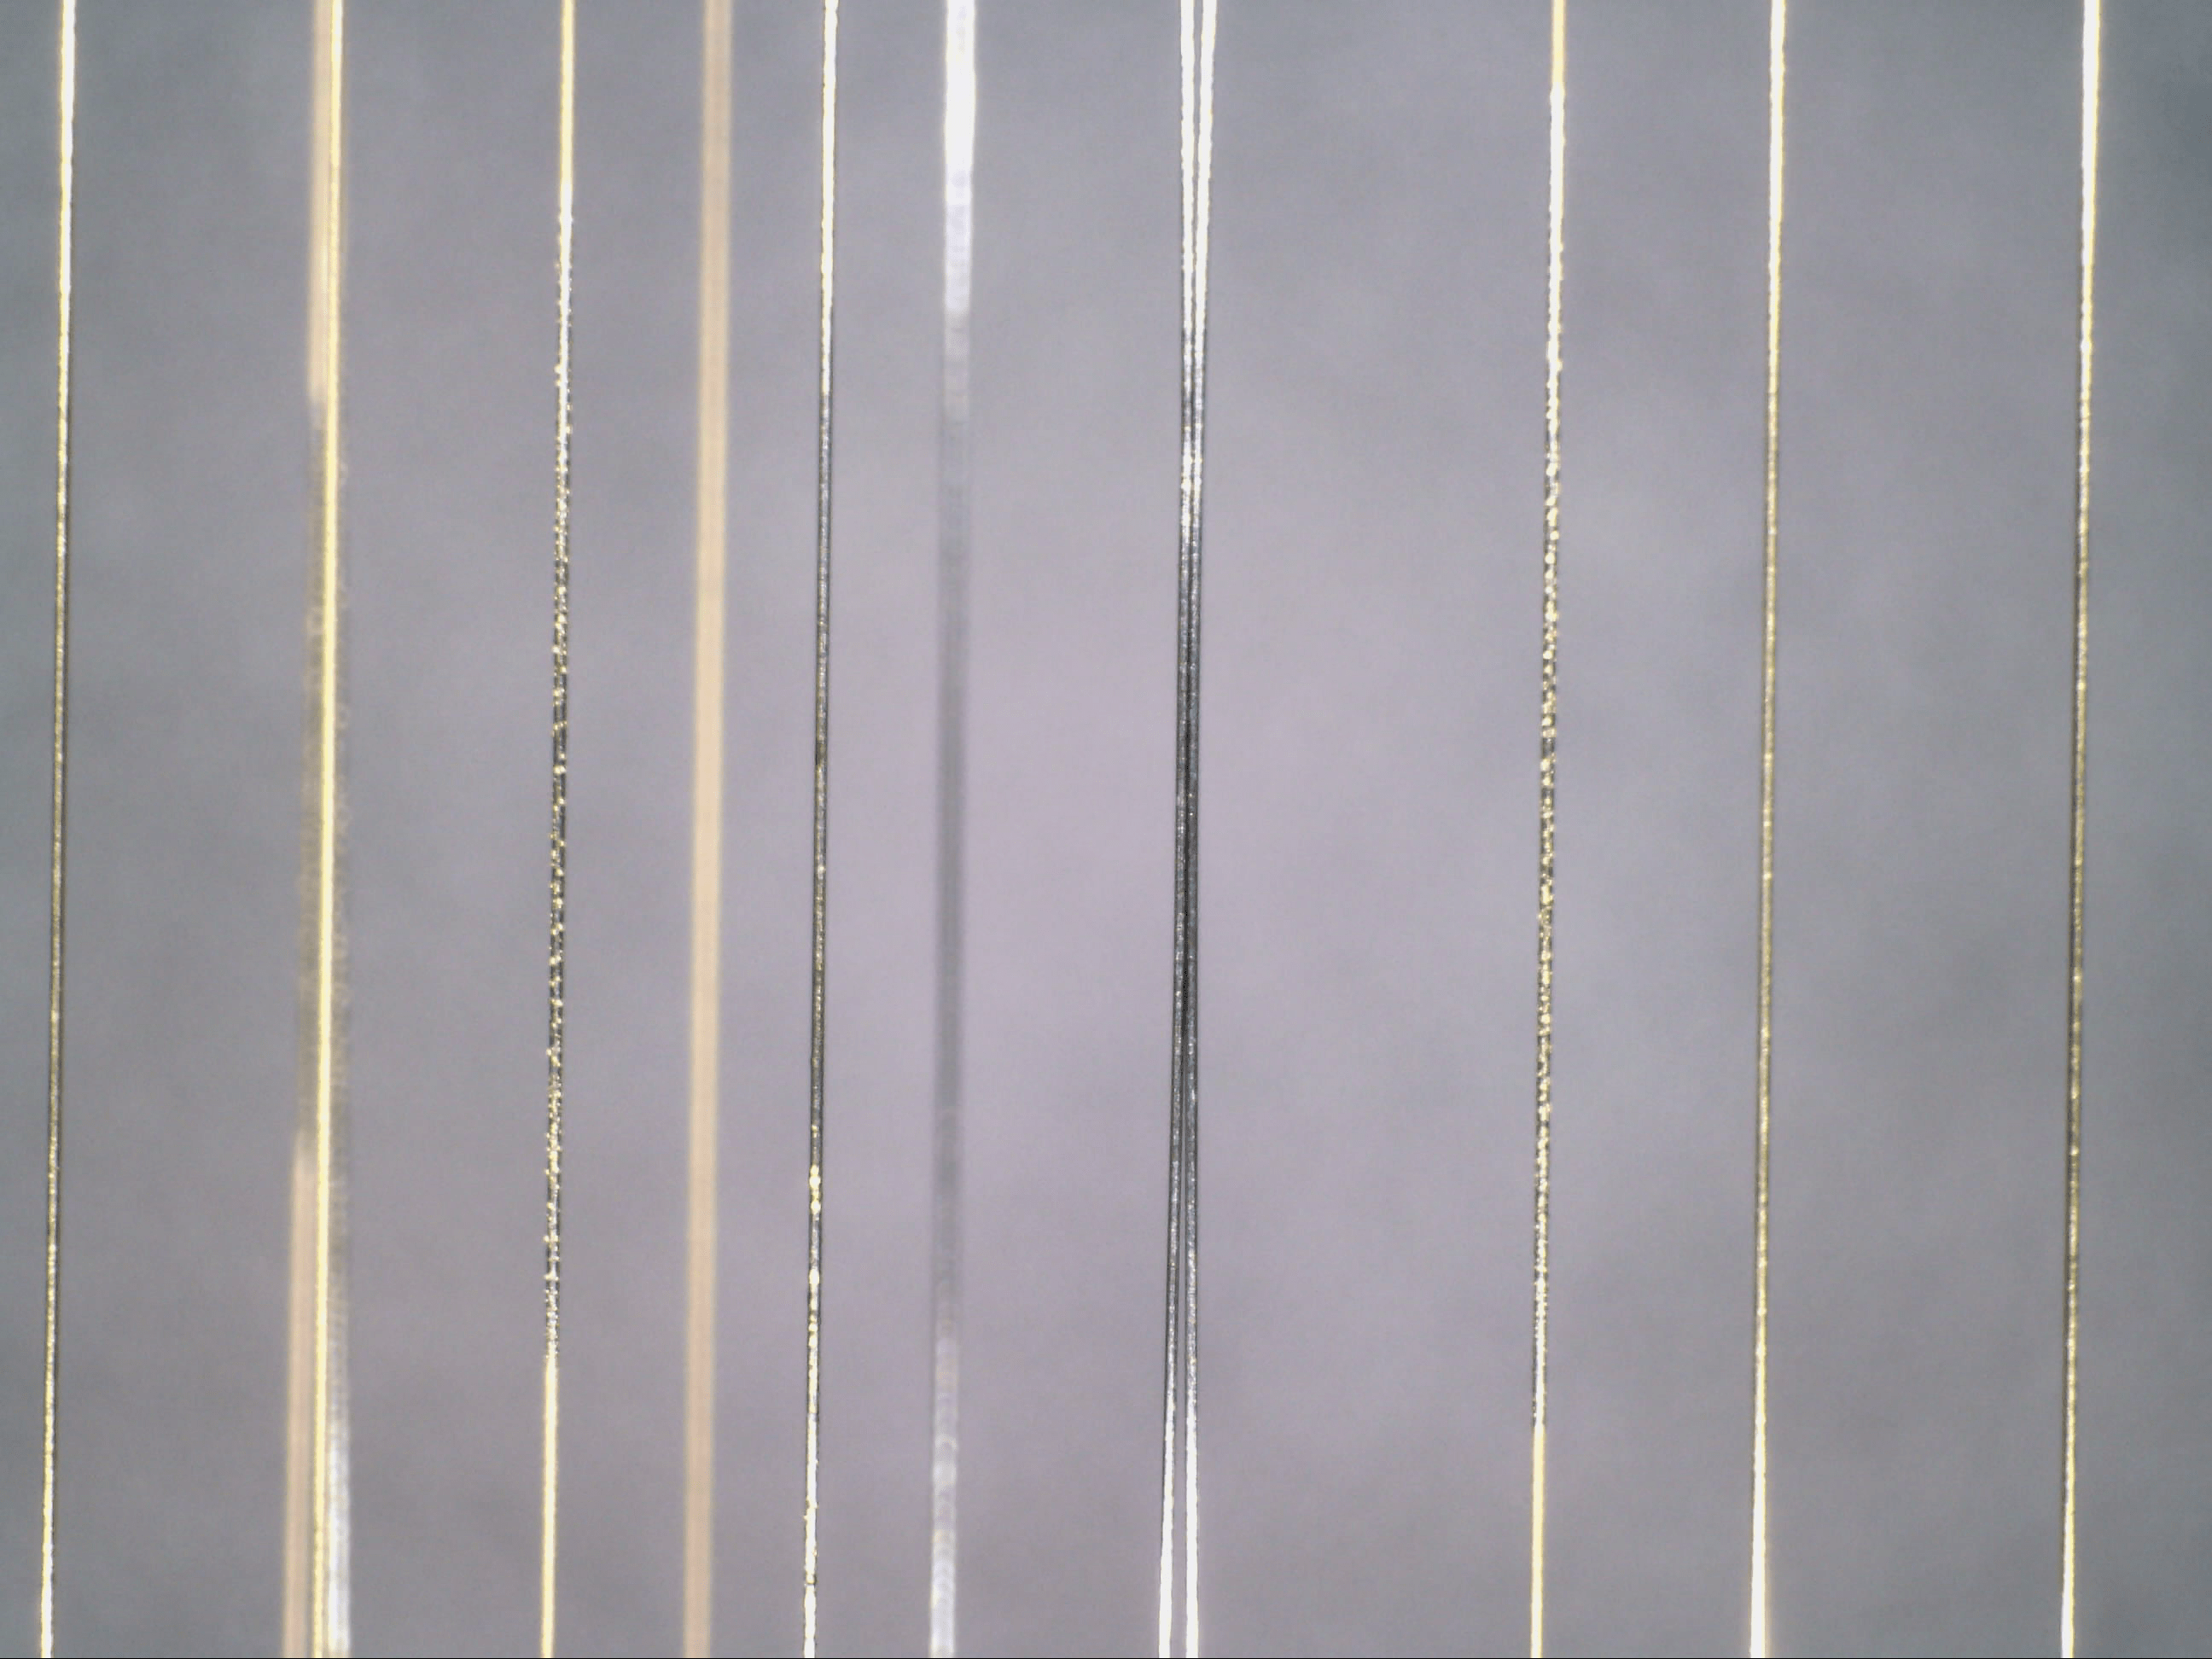
\includegraphics[width=\textwidth]{SEMgridDamage/GridDamage2.png}
    \end{subfigure}
    \caption{SEM Grid used at Linac4, in L4T Line.  }
    \label{fig:SEMLinac4damage}
\end{figure}

\section{The heat equation}
\label{sec:HeatEq}

To understand the temperature variation of thin target detectors during operation, we need first to introduce the different processes that collaborate in this thermal evolution. In our case, the temperature variation can be described as: 
\begin{equation}
    \left(\frac{\partial T}{\partial t}\right)_{tot} = \left(\frac{\partial T}{\partial t}\right)_{Ht} - \left(\frac{\partial T}{\partial t}\right)_{Rd} - 
                 \left(\frac{\partial T}{\partial t}\right)_{Cd} - \left(\frac{\partial T}{\partial t}\right)_{Th} - \left(\frac{\partial T}{\partial t}\right)_{Sub}
    \label{eq:HeatBalance}
\end{equation}

Where the term with sub-index Ht represents the beam heating, and it is accompanied by several cooling processes such as radiative cooling (Rd), conduction cooling (Con), thermionic cooling (Th) and sublimation cooling (Sub). Because in our case this thermal model is going to be used for applications in ultra-high vacuum conditions ($10^{-6} - 10^{-9}$ mbar), cooling phenomena such as convection are not considered. 

To simplify the notation, the dependences of the different terms have not been included in equation \ref{eq:HeatBalance}. The temperature depends on the time (t) and on the spatial coordinates (x,y). Due to the thin target nature of the detectors, the coordinate (z) along the beam axis will not be considered. 

\subsection{Target Heating (Ht)}
\label{sec:BeamHeating}

Beam-induced detector heating can be traced down to two possible phenomena: 

\begin{itemize}
    \item Direct Beam Energy Deposition: It is related to nuclear and atomic interactions of the beam of particles with the material of the detector. 
    \item Indirect Electromagnetic Coupling: This is related to the energy exchange due to electromagnetic coupling between the beam of particles and the detector. 
\end{itemize}

Indirect electromagnetic coupling is a phenomenon that can be heavily mitigated by properly designing the detector geometry, and will not be covered in this work. If it is of the reader interest, a detailed description of this phenomenon can be found in \parencite[][]{ref:ElectroHeating}. One can describe the temperature variation due to direct energy deposition as follows: 
\begin{equation}
    \left(\frac{\partial T}{\partial t}\right)_{Ht} = \frac{N (x,y,t)}{V\cdot Cp(T)\cdot \rho (T)}\cdot \frac{dE}{dx}
\end{equation}

Where V, Cp(T) and $\rho (T)$ are the volume, specific heat and density of the detector's material. $dE/dx$ is the single particle energy deposition, which was explained in Chapter \ref{ch:BeamMatterInter}. N(x,y,t) refers to the surface density of beam particles reaching a point in space (x,y) at time t. This concept can be generalized to any particle distribution. However, in most cases, the beam of particles can be described as a Gaussian distribution. In that case, N(x,y) can be described as: 

\begin{equation}
    N(x,y) = \frac{N_{Tot}}{2 \pi \sigma_x \sigma_y}\cdot exp \left(
              -\frac{1}{2}\left(\frac{x-x_0}{\sigma_x}\right)^2 - \frac{1}{2}\left(\frac{y - y_0}{\sigma_y}\right)^2\right)
\end{equation}

Here $x_0$ and $y_0$ represent the coordinates of the beam centroid and $\sigma_x$ and $\sigma_y$ represent the standard deviation of the normally distributed beam of particles. $N_{tot}$ is the total number of particles (per unit time) in the particle beam. The temporal distribution can be approximated as a pulse train function. This means: 

\begin{equation}
    \begin{cases}
      N(x,y,t) = N(x,y) \mspace{30mu} if\mspace{18mu}Beam = Yes \\
      N(x,y,t) = 0 \mspace{80mu} if \mspace{18mu}Beam = No 
    \end{cases}
\end{equation}

\subsection{Radiative Cooling (Rd)}
\label{sec:RadiativeCooling}

Radiative cooling occurs due to heat transfer by thermal radiation carried by electromagnetic waves \parencite[][]{ref:RadiativeCooling}. In vacuum,  or in materials that allow the transmission of electromagnetic waves, radiation cooling might be of great importance. 

Radiative cooling is a surface effect, and it depends on the surface characteristics and its temperature.  The net temperature variation from a surface S at a temperature T to a surrounding large enclosure at temperature $T_0$ can be described by Stephan-Boltzman's law as follows: 

\begin{equation}
    \left( \frac{\partial T}{dt} \right)_{Rad} = \frac{S\cdot \sigma_{SB}\cdot \epsilon(T)\cdot \left(T(x,y,t)^4 - T_0^4\right)}{Cp(T)\cdot V \cdot \rho(T)}
\end{equation}

Where $\sigma_{Sb}$ is the Stephan-Boltzmann constant and $\epsilon$ is the emissivity of the material. Emissivity is a measure of the efficiency with which a surface emits thermal energy and it is defined as the ratio of the energy radiated from a material's surface to that radiated from a perfect emitter, known as black-body. A more detailed description of the emissivity can be found in chapter \ref{ch:EmissivityMeas}. 

\subsection{Conduction Cooling (Cd)}
\label{sec:ConductionCooling}

Thermal conduction in solids or static fluids \parencite[][]{ref:ConductionCooling} occurs as soon as a spatial temperature gradient exists. The carriers of the energy transfer can be molecules, atoms, electrons and phonons. The rate of change due to conduction can be described by Fourier's equation as follows: 

\begin{equation}
    \left( \frac{\partial T}{\partial t} \right)_{Cond} = \alpha (T) \left( \frac{\partial^2 T}{\partial x^2} + \frac{\partial^2 T}{\partial y^2} \right)
\end{equation}

$\alpha(T)$ is called the thermal diffusivity of the medium and it measures the rate of heat transfer in a material from the hot end to the cold end. It has SI units of $m^2 /s$. It can be calculated as follows: 
\begin{equation}
    \alpha(T) = \frac{k(T)}{\rho(T)Cp(T)}
\end{equation}

Where k(T) is defined as the thermal conductivity of the material (W/mK), which is the measure of the capability of the material to conduct heat. In general, metals have high thermal conductivity and gases have low thermal conductivity. 

\subsection{Thermionic Cooling (Th)}
\label{sec:ThermionicCooling}

Thermionic emission was in Section \ref{sec:ThermoCurrent}. As was said before, thermionic emission is a process by which free electrons are emitted from the surface of a metal when they gain enough thermal energy to overcome the work function. These thermionic electrons take with them some energy, and this contributes to the thermal cooling \parencite[][]{ref:ThermoCooling}. The temperature variation due to thermionic emission can be described as: 

\begin{equation}
    \left(\frac{\partial T}{\partial t}\right)_{Th} = S\cdot \left( \phi +2K_B T\right)\cdot \frac{J_{Th}(T)}{C_p(T)\cdot V \cdot \rho(T)}
\end{equation}

Where $\phi$ is the work function of the material. $K_B$ is Boltzmann constant. $J_{th} (T)$ was described in section \ref{sec:ThermoCurrent} can be written as: 
\begin{equation}
    J_{th} (T) = A_R \cdot T^2\cdot exp\left(-\frac{\phi}{K_B T}\right)
\end{equation}

\subsection{Sublimation Cooling (Sub)}
\label{sec:SublimationCooling}

Sublimation is a process in which a solid changes into a gas without passing through the liquid phase. To sublimate a substance, certain energy must be provided. We will call this energy $H_{sub}$, and it must be sufficient to break the intermolecular forces holding the solid together. Usually it is expressed in (KJ/mol) and can be found in the literature. Similar to the thermionic case, the newly formed gas molecules will escape the material, and the energy given to them for transforming their estate contributes to the overall cooling of the detector \parencite[][]{ref:SublimationCooling}. This sublimation cooling can be written as: 

\begin{equation}
    \left(\frac{\partial T}{\partial t}\right)_{Sub} = H_{sub}\cdot n(T)
\end{equation}

n(T) is the material sublimation rate. Following the same procedure as \parencite[][]{ref:SubRate}, one can determine an upper limit of this sublimation rate. For that one needs to assume the following: 

\begin{itemize}
    \item No atoms leaving the boundary layer return to the hot surface. 
    \item A thin boundary layer over the hot material surface is at equilibrium with the substance sublimation pressure ($P_{vap}$) for temperature $T_{vap}$. 
    \item This thin layer of gas is considered to be an ideal gas. 
\end{itemize}

With these approximations, the amount of sublimated material per unit of time can be expressed as: 
\begin{equation}
    d_{sub} = \frac{1}{2}v_{vap}\cdot \rho_{vap} \cdot \rho_{c}
    \label{eq:SubMaterial}
\end{equation}

$v_{vap}$ is the velocity of the vapor particles. From an ideal gas theory, we know that the average velocity of gas particles in a hemisphere can be described as follows: 

\begin{equation}
    v_{vap} = \frac{1}{2}\cdot \sqrt{\frac{8k_B T_{vap}}{m \pi}}
\end{equation}

Where m is the mass of the material particle. In equation \ref{eq:SubMaterial}, $\rho_{vap}$ refers to the vapor density in the equilibrium layer and can be expressed using the formula: 

\begin{equation}
    rho_{vap} = \frac{m_{mol} T_{std}}{V_{mol} P_{atm}}\cdot \frac{P_{vap}(T_{vap})}{T_{vap}}
\end{equation}

Where $P_{atm}$ is the atmospheric pressure ($10^5$ Pa), $V_{mol} = 22.4$ $dm^3$ is the molar volume of an ideal gas at the standard temperature $T_{std} = 273$ K. The vapor pressure highly depends on the maximum temperature of the material, and thus, the total amount of sublimated material will highly depend on the temperatures reached. 

\section{Numerical Approximation to the heat equation.}
\label{sec:NumericalMethod}

Putting together all the concepts from the previous section, we can re-write equation \ref{eq:HeatBalance} as follows: 
\begin{multline}
    \left(\frac{\partial T}{\partial t}\right)_{Tot} = 
    \frac{N(x,y,t)}{V\cdot Cp(T) \cdot \rho (T) }\cdot \frac{dE}{dx} \\
    - \frac{S\cdot \sigma_{SB}\cdot \epsilon(T)\cdot \left(T^4 - T_0^4\right)}{Cp(T)\cdot V \cdot \rho(T)} 
        -\alpha (T) \left( \frac{\partial^2 T}{\partial x^2} + \frac{\partial^2 T}{\partial y^2} \right)  \\
        - S\cdot \left( \phi +2K_B T\right)\cdot \frac{J_{Th}(T)}{C_p(T)\cdot V \cdot \rho(T)} - H_{sub} \cdot n(T)
    \label{eq:ExplicitHeatEq}
\end{multline}

This is an evolutionary, non-linear, second order, partial differential equation (PDE). In this work, this equation is treated numerically. The subject of PDEs and how to solve them is very broad. An enormous number of different numerical techniques to solve non-linear or quasi-linear PDEs exist. For an outstanding introduction to this world, I recommend the reader to check \parencite[][]{ref:NumericalMethodBook}, where a small number of tools are introduced forming a solid basis for the understanding of the subject. 

In this document, we will focus on the classical theory of finite differences. The main idea in the calculus of finite differences is to replace derivatives with linear combinations of discrete function values. One assumes the numerical solution is known only at a finite number of points (or nodes) in the physical domain. Figure \ref{fig:SpaceDiscret} shows an example of the spatial discretization of a homogeneous body. 

\begin{figure}[h]
    \centering
    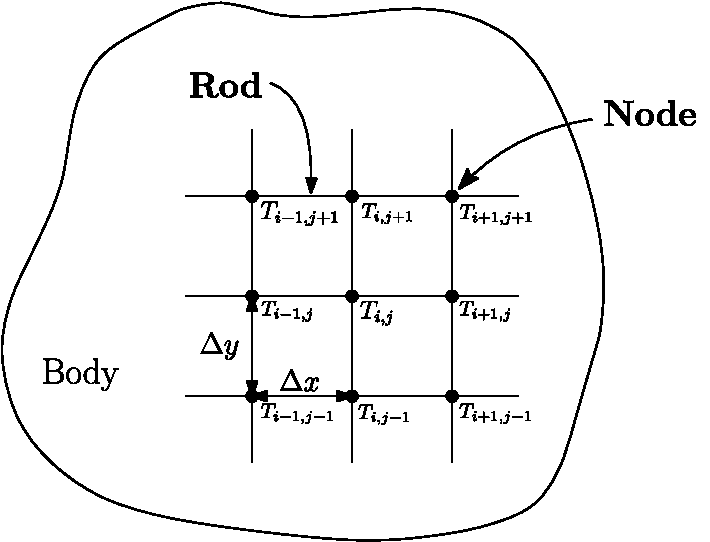
\includegraphics[width=0.5\columnwidth]{SpaceDiscretization/SpaceDiscretization.pdf}
    \caption{Space discretization of a homogeneous body.}
    \label{fig:SpaceDiscret}
\end{figure}

The parameters $\Delta x$ and $\Delta y$ indicate the local distance between adjacent points in space, and in our case, they are considered to be uniform throughout the mesh. Increasing the number of nodes in the mesh (reducing $\Delta x , \Delta y$) increases the resolution and the accuracy of the numerical solution. However, it increases computational costs.

Every node in the grid has a temperature and can exchange heat with its neighbors through a heat conducting rod. The sub-indexes i, j are used to refer to nodes in the physical space.  $T_{i,j}$ refers to the temperature in the position $x_i , y_j$.

Because the temperature of the system changes a function of time, the numerical solution of the PDE requires also time discretization. Figure \ref{fig:TimeDiscret} shows a schematic representation of the time discretization of a strip of material. The time nodes are referred to with the super-index m, so that $T^{m}$ corresponds to the temperature at the time instant  $t^m$.  $\Delta t$ refers to the difference between time nodes. This distance was also considered to be equidistant, however, two different time constants were considered, one for the heating time ($\Delta {t}_{heat}$) and one for the cooling period ($\Delta t_{Coold}$). In most applications, the beam of particles is pulsed, and the beam pulse length is much shorter than the period without beam. 

\begin{figure}[h]
    \centering
    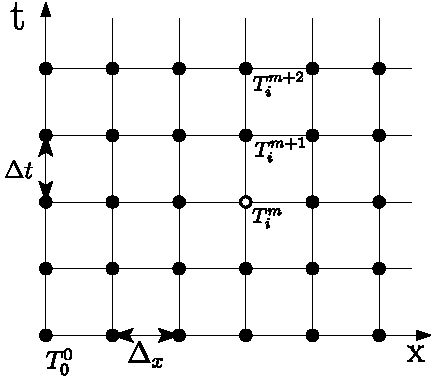
\includegraphics[width=0.4\columnwidth]{TimeDiscretization/TimeDiscret.pdf}
    \caption{Time discretization of the material rod.}
    \label{fig:TimeDiscret}
\end{figure}

\subsection{Finite Differences Schemes}
\label{sec:FD}

Working with the full heat equation (eq. \ref{eq:ExplicitHeatEq}) can result in a very cumbersome notation. The one-dimensional case of a thin rod with only radiative and conduction cooling will be considered for this explantion. The simplified equation that we will treat here is: 

\begin{equation}
    \frac{\partial T(x,t)}{\partial t} = 
        H(x,t,T)
        - A(T) \left(T(x,y)^4 - T_0^4\right)
            -\alpha (T)  \frac{\partial^2 T(x,t)}{\partial x^2}   
            \label{eq:SimpleHeating}
    \end{equation}

Where H(x,t) refers to the heating term. A(T) can be written as: 

\begin{equation}
    A(T) = \frac{S\cdot \sigma_{SB}\cdot \epsilon(T)}{Cp(T)\cdot V \cdot \rho(T)}. 
\end{equation}

At any instant of time, one has access only to the values of the temperature at the afore-mentioned nodes ($T^{m}_{ij}$). The objective now is to obtain an approximation of $\partial T/dt$, $\partial^2 T,\partial x^2$ and $\partial^2 T/\partial y^2$ in those nodes by only knowing the information provided by the other nodes. Using different combinations of the mesh points results in different schemes. In the following, three of these schemes will be introduced. For a more detailed description of these methods, one can check the reference \parencite[][]{ref:FiniteDifference}.

\subsubsection{Forward in Time, Centered in Space (FTCS)}

This scheme approximates the time derivative with a forward difference: 

\begin{equation}
    \left. \frac{\partial T}{\partial t}\right|_{t^{m+1},x_i}  = \frac{T^{m+1}_i - T^m_i}{\Delta t} +  \mathcal{O} \left( \Delta t \right)
 \end{equation}

And for $\partial^2 T/ \partial x^2$ a central difference approximation is used. 

\begin{equation}
    \left. \frac{\partial^2 T}{\partial x^2}\right|_{x_i} = \frac{T^{m}_{i-1}-2T^m_{i}+T^m_{i+1}}{\Delta x^2}+\mathcal{O}\left(\Delta x^2 \right)
    \label{eq:CD}
\end{equation}

The expression $\mathcal{O}(\Delta t)$ is telling us, that the local truncation error, in this case, is proportional to the time step size, while $\mathcal{O}(\Delta x)$ indicates that the truncation error reduces quadratically with the spatial step size. 

\begin{figure}[h]
    \centering
    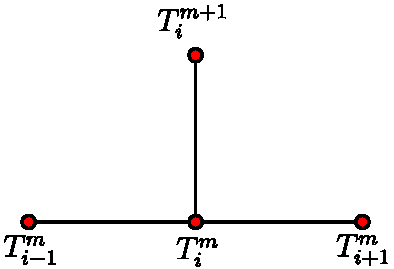
\includegraphics[width=0.35\columnwidth]{Stencils_FiniteDifferences/FTCS.pdf}
    \caption{Stencil for the Forward Time, Central Space finite difference method.}
    \label{fig:StencilFTCS}
\end{figure}

The stencil of this method can be found in figure \ref{fig:StencilFTCS}. This method calculates the state of the system at a later time from the state of the system at the current time. It is considered to be an explicit method. Introducing these approximations in equation \ref{eq:SimpleHeating} one obtains:

\begin{equation}
    \frac{T^{m+1}_i - T^m_i}{\Delta t} = H^m_i - A_i^m \left((T_i^m )^4 - (T_0)^4\right) +\alpha_i^m    \frac{T^{m}_{i-1}-2T^m_{i}+T^m_{i+1}}{\Delta x^2}
\end{equation}

After a little bit of algebra, this equation can be written in a matrix form.

$$
\begin{bmatrix}
         1 & 0 & 0 & 0 & 0 & 0 \\
         r^m_1 & \left(1-2r^m_1\right) & r^m_1 & 0 & 0 & 0 \\ 
         0 & r & \left(1-2r^m_1\right) & r^m_1 & 0 & 0 \\ 
         0 & 0 & \ddots & \ddots & \ddots & 0 \\
         0 & 0 & 0 & r^m_1 & \left(1-2r^m_1\right) & r^m_1 \\
         0 & 0 & 0 & 0 & 0 & 1 
     \end{bmatrix}
\begin{bmatrix}
         T^m_0  \\
         T^m_1 \\ 
         T^m_2  \\ 
         \vdots \\
         T^m_{N-1} \\
         T^m_N 
     \end{bmatrix}
     =
     \begin{bmatrix}
         T^{m+1}_0 + g(T^m_0) \\
         T^{m+1}_1 + g(T^m_1)\\ 
         T^{m+1}_2 + g(T^m_2)\\ 
         \vdots\\ 
         T^{m+1}_{N-1} + g(T^m_{N-1})\\
         T^{m+1}_{N} + g(T^m_{N}) 
     \end{bmatrix}
$$

With $r^m_i = \alpha^m_i \cdot \Delta t/ \Delta x^2$. And with g(T) including all the non-linear terms of the equation. In a more simplified way: 

\begin{equation}
    D_{FTCS}\cdot T^{m} = T^{m+1}+g(T^m)
\end{equation}

This is a relatively simple method to implement, as the values of $T_i^{m+1}$ can be updated independently of each other. However, the FTCS method can yield unstable solutions that can oscillate and grow if $\Delta t$ is too large. To ensure stability: 

\begin{equation}
    r = \alpha\cdot \frac{\Delta t}{\Delta x} < \frac{1}{2}
    \label{eq:rstab}
\end{equation}

See \parencite[][]{ref:proveR1} and \parencite[][]{ref:proveR2} for a proof that equation \ref{eq:rstab} gives the stability condition for FTCS. 

\subsubsection{Backwards in Time, Centered Space (BTCS)}

In this case, a backward in time difference is used to approximate the time derivative while a central space scheme is used for the spatial derivative: 

\begin{equation}
    \left. \frac{\partial T}{\partial t} \right|_{t^{m+1},x_i} = \frac{T^m_i - T^{m-1}_i}{\Delta t}+\mathcal{O}(\Delta t)
\end{equation}

As in the previous case, the full equation can be represented in a matrix form: 

$$
\begin{bmatrix}
         b_0 & c_0 & 0 & 0 & 0 & 0 \\
         a_1 & b_1 & c_1 & 0 & 0 & 0 \\ 
         0 & a_2 & b_2 & c_2 & 0 \\ 
         0 & 0 & \ddots & \ddots & \ddots & 0 \\
         0 & 0 & 0 & a_{N-1} & b_{N-1} & c_{N-1} \\
         0 & 0 & 0 & 0 & a_N & b_N 
     \end{bmatrix}
\begin{bmatrix}
         T^m_0  \\
         T^m_1 \\ 
         T^m_2  \\ 
         \vdots \\
         T^m_{N-1} \\
         T^m_N 
     \end{bmatrix}
     =
     \begin{bmatrix}
         d_0 + g(T^m_0) \\
         d_1 + g(T^m_1)\\ 
         d_2 + g(T^m_2)\\ 
         \vdots\\ 
         d_{N-1} + g(T^m_{N-1})\\
         d_{N} + g(T^m_{N}) 
     \end{bmatrix}
$$

Where the coefficients are:

\begin{equation}
    \begin{gathered}
        a_i = -r^m_{i-1} \\
    b_i = 1 + 2r^m_{i}\\
    c_i = - r^m_{i+1} \\
    d_i = T^{m-1}_i + g(T_i^m)
    \end{gathered}
\end{equation}

Figure \ref{fig:StensilBTCS} shows the stencil representation of this method. In this case, we are dealing with an implicit method. To find the temperature in the time step m one must solve an equation involving the current state of the system (m) and the previous state (m-1). 

\begin{figure}[h]
    \centering
    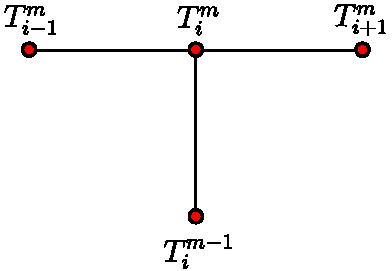
\includegraphics[width=0.35\columnwidth]{Stencils_FiniteDifferences/BTCS.pdf}
    \caption{Stencil for the Backwards in time, Central in space finite difference method.}
    \label{fig:StensilBTCS}
\end{figure}

\subsubsection{Crank-Nicolson}

To improve the temporal truncation error, the Crank-Nicolson scheme approximates the spatial derivative by the average of the central difference scheme, evaluated in the current (m) and the previous (m-1) time steps: 

\begin{equation}
    \frac{T^m_i - T^m_i}{\Delta t} = g(T^m_i) + \frac{\alpha^m_i}{2}\left[ 
          \frac{T^m_{i-1}- 2 T^m_i + T_{i+1}^m}{\Delta x^2} + \frac{T^{m-1}_{i-1}-2T^{m-1}_i+T_{i+1}^{m-1}}{\Delta x^2}
    \right] 
\end{equation}

The stencil representation of this method is shown in Figure \ref{fig:StencilCrNic}. This method is implicit, like the BTCS method. However, it accomplishes a truncation error $\mathcal{O}(\Delta t^2)$ without overcomplicating the implementation. The matrix representation is the same as in the BTCS case, but with the following coefficients:

\begin{equation}
    \begin{gathered}
        a_i = -r^m_{i-1}/2 \\
        b_i = 1 + r^m_{i}\\
        c_i = - r^m_{i+1}/2 \\
        d_i = a_i T_{i-1}^{m-1} + (1 + a_i + c_i) T^{m-1}_{i} + c_i T_{i+1}^{m-1} + g(T_i^m)
    \end{gathered}
\end{equation}

\begin{figure}[h]
    \centering
    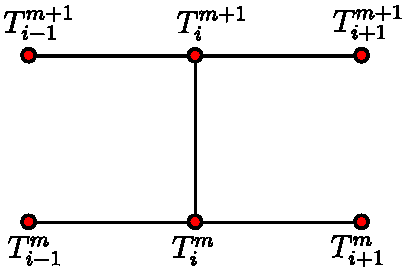
\includegraphics[width=0.35\columnwidth]{Stencils_FiniteDifferences/CrkNic.pdf}
    \caption{Stencil for the Crank-Nicolson finite difference method.}
    \label{fig:StencilCrNic}
\end{figure}

\subsection{Initial and Boundary Conditions}

Due to the time-dependent part of our equation, we need an initial condition. In this case, this refers to the temperature of the system at time $t^0$. Unless specified otherwise, a constant temperature $T_{i,j}^0 = 300 (K)$ will be considered.

At each time step, because of the spatial dependence of the equation, some boundary conditions need to be specified. Here the so-called Dirichlet boundary conditions are considered. For the one-dimensional case, these conditions can be written as follows: 
\begin{equation}
    \begin{cases}
      T(0,t) = 300 \mspace{30mu} (K) \\
      T(L,t) = 300 \mspace{30mu} (K) 
    \end{cases}
\end{equation}

Where L refers to the length of the one-dimensional rod. In the 2D case, these conditions would indicate that all the borders of the foil are in contact with a thermal sink at 300 (K). 

\subsection{The Non-Linear Problem}

In the previous sections, g(T) was described as the non-linear term. The explicit expression is: 
\begin{equation}
    g(T) = \frac{N(x,t)}{V\cdot Cp(T)\cdot \rho(T)}\frac{dE}{dz} - \frac{S\cdot \sigma_{SB}\epsilon(T)\cdot \left( T(x,t)^4 - T_0^4\right)}{V\cdot Cp(T)\cdot \rho(T)}
\end{equation}

In the case with no heating and no radiative cooling, g(T) = 0. This case yields to the diffusion equation. In this scenario, the systems of equations presented in the previous section can be easily solved by techniques such as Gaussian elimination methods, LU factorization, etc. More information about those methods can be found in \parencite[][]{ref:AlvaroBook}. 

$g(T) \neq 0$ implies that now, at each time step, one has to solve a system of non-linear equations. This is still solvable numerically, but it implies using other numerical techniques such as Newton's method for non-linear systems \parencite[][]{ref:AlvaroBook}. At every time step, one must guess an approximate solution and compute the Jacobian matrix. Which can be computationally expensive and cumbersome. By default, instead of considering the full equation, each term of the equation is considered separately and then added together. For equation \ref{eq:SimpleHeating} this would mean solving the following: 

\begin{equation}
    \frac{\partial \Delta T_{Ht} (x,t)}{\partial t} = H(x,t,T)
\end{equation}
\begin{equation}
    \frac{\partial \Delta T_{Rad} (x,t)}{\partial t} = A(T) \left(T(x,y)^4 - T_0^4\right)
\end{equation}
\begin{equation}
    \frac{\partial \Delta T_{Con}}{\partial t} = \alpha(T)\frac{\partial^2 T(x,t)}{\partial x^2}
\end{equation}

The total temperature variation is then calculated as: 

\begin{equation}
    \Delta T_{tot} = \Delta T_{Ht} - \Delta T_{Rd} - \Delta T_{Con}
\end{equation}

\section{The two-dimensional problem}

The biggest difference in the two-dimensional case is the conduction term on the heat equation. Each point in space is now connected to four other points, that is, there is conduction along four rods. For the two-dimensional case, a five-point finite difference formulation is used \parencite[][]{ref:FiniteDifference}. Taking the simplified case of the 2D diffusion equation: 
\begin{equation}
    \frac{\partial T(t,x,y)}{\partial t} = \alpha (T) \left(\frac{\partial^2 T}{\partial x^2}+\frac{\partial ^2 T}{\partial y^2}\right)
\end{equation}

One could write the FTCS formulation as follows: 
\begin{equation}
    \frac{T_{i,j}^{m+1} - T_{i,j}^{m}}{\Delta t} = \alpha(T_{i,j}^{m}) \left( \frac{T_{i-1,j}^{m} -2T_{i,j}^{m}+T_{i+1,j}^{m}}{\Delta x^2} +  \frac{T_{i,j-1}^{m}-2T_{i,j}^{m}+T_{i,j+1}^{m}}{\Delta y^2} \right)
\end{equation}

Similarly, this could be applied to the BTCS and Crank-Nicolson formulations. The same procedure to transform this into a system of equations, and solve it numerically, can also be followed. 

\section{Importance of Cooling Effects}

The most accurate simulation is obtained when all the cooling mechanisms indicated in equation \ref{eq:HeatBalance} are considered. However, if simulation speed is what matters, a faster simulation can be run by ignoring certain cooling mechanisms. Particularly, conduction cooling is the most time-consuming effect. Figure \ref{fig:CoolingComparison} shows how much each cooling mechanism contributes to the total cooling as a function of the temperature. This figure was calculated for a 30 $\mu m$ Graphite wire. It might differ slightly for different materials and geometries. 

\begin{figure}[h]
    \centering
    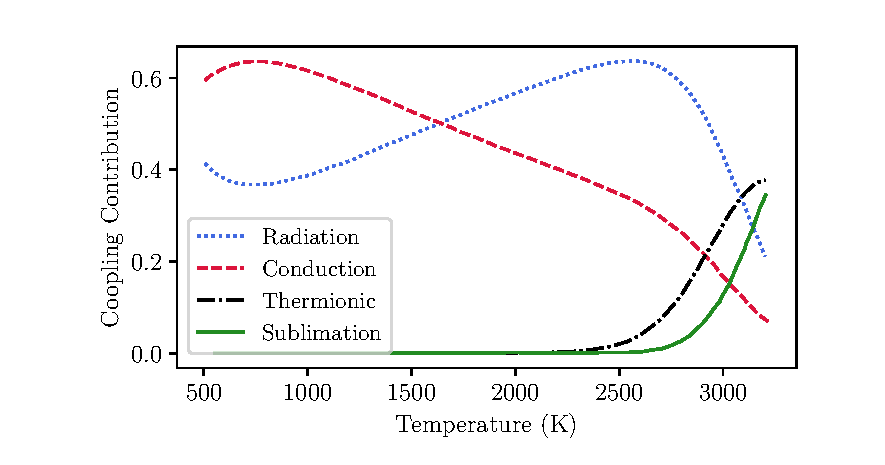
\includegraphics[width=1.0\columnwidth]{PlotCoolingImportancfe/CoolingImpo.pdf}
    \caption{Relative importance of the different cooling mechanisms as a function of the temperature.}
    \label{fig:CoolingComparison}
\end{figure}

From this figure, one can observe how radiation cooling is the predominant mechanism throughout the biggest temperature range. For a thin wire, conduction cooling plays a very important role at lower temperatures while thermionic and sublimation cooling are important only at very high temperatures. If there is some a-priory knowledge of the expected temperature range, or simply a fast upper limit of the maximum temperature is needed, various cooling processes can be deliberately eliminated for speed purposes.

\section{PyTT}
\label{sec:GUI}

The simulation program was implemented using Python 3.6.9. The latest version of the code can be found at \parencite[][]{ref:GitAra}. As aforementioned, the main objective of this code is to quickly obtain an estimation of the maximum temperature reached by thin target detectors when interacting with the beam of particles. Additionally, the code also needed to be easy to use by people who aren't particularly familiar with python or numerical techniques. For that, a user-friendly interface was implemented.

\begin{figure}[h]
    \centering
    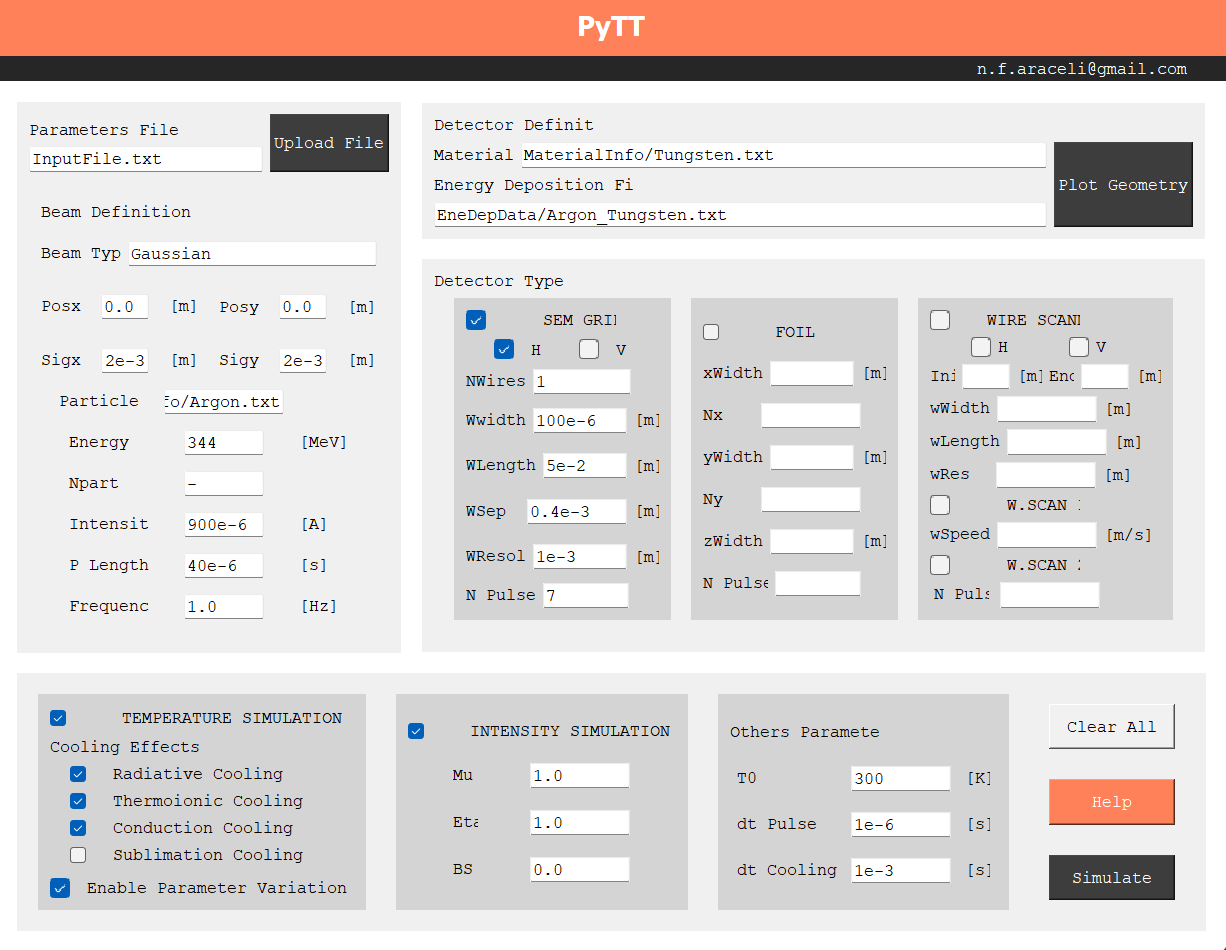
\includegraphics[width=0.9\columnwidth]{PyTT_GUI/PyTTScreanshot.png}
    \caption{Graphical User-Friendly interface of PyTT code.}
    \label{fig:UserFriendly}
\end{figure}

Figure \ref{fig:UserFriendly} shows a screenshot of the GUI. The implementation of the code and its usage will not be discussed in this document. Just the main description of its functionalities will be given. 

\begin{enumerate}
    \item Variety of Beam Conditions: To simulate a variety of cases, the program allows the user to choose several beam parameters. For example, the particle or ion type and energy, the spatial and temporal distribution, and the repetition frequency of the particle beam. 
    \item Variety of Detector Materials: The material of the detector can be chosen freely, by either selecting one of the already given materials or by easily creating one's own. 
    \item Type of thin target detectors: The program can simulate SEM grid detectors, Thin foils and Wire scanners. For the wire scanners, both fast and slow wire scanners can be considered. 
    \item Choosable simulation Parameters:  Several simulation parameters (Such as space-time discretization parameters, simulation length, thermal effects, parameter temperature dependence, etc.) Can be easily selected at the user's convenience. 
    \item Intensity Simulation: The program includes an intensity simulation module that includes the model explained in chapter \ref{ch:CurrentModeling}. This calculates the current generation in the detector during operation. 
\end{enumerate}

Results like the maximum temperature in the detector as a function of time are provided by default. Figure \ref{fig:GUIResults} shows an example of the simulated output. However, using the output files produced by the simulation, some additional results can be attained. These can include, spatial thermal distributions, the relative importance of the different cooling methods, the evolution of material properties during simulation, intensity distribution, etc. 

\begin{figure}[h]
    \centering
    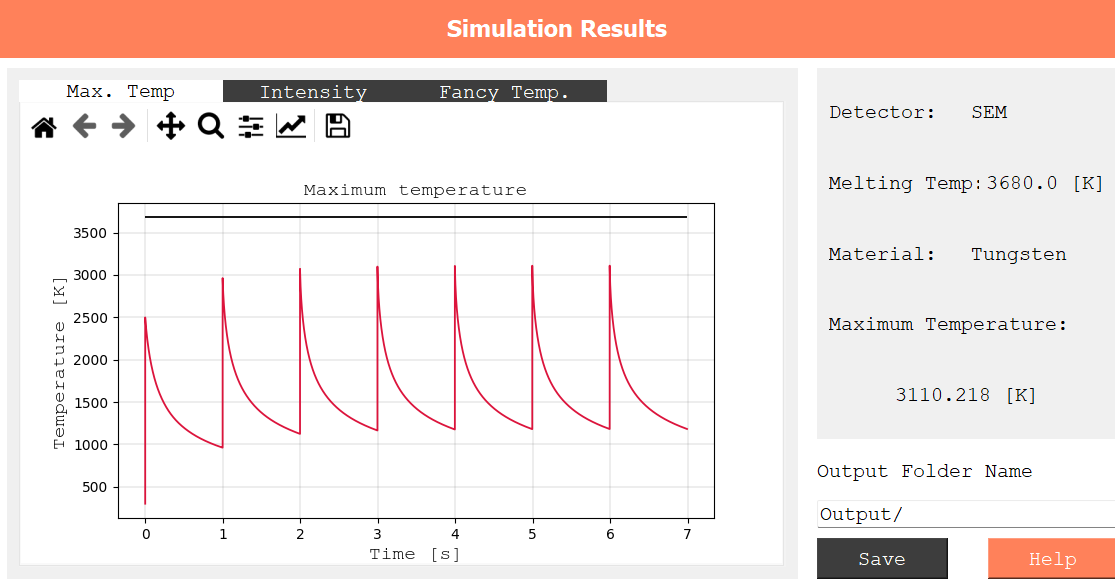
\includegraphics[width=0.9\columnwidth]{PyTT_GUI/PyTTresults.png}
    \caption{Example of output visualization GUI.}
    \label{fig:GUIResults}
\end{figure}

The program has been optimized for it to be used by the python interface. However, it can also be launched by a stand-alone executable for windows systems. It can also be used without the GUI, which allows for easy paralelization and automatization. A more detailed description of how to use the code can be found in the user manual, accessible through the help button in the GUI, or directly in the HelpFolder.

\section{Model uncertainties}
\label{sec:ModelUnc}

As with all models, the approximations done along the way induce uncertainties in the final results. The simulation results highly depend on our knowledge of the simulation case. That is, the better one can describe the experimental situation, the more accurate the simulated results. A lot of different parameters are involved in this description. To simplify the study one can divide these parameters into two categories: Beam Parameters and Material Properties. 

\subsection{Beam Parameter Uncertainties.}

These parameters are the ones used to describe the spatial and temporal distribution of the beam of particles. If we take as an example the case of a Gaussian beam, those parameters would be: beam size ($\sigma_x , \sigma_y$), beam position, Intensity, pulse length, repetition rate, etc. 

To calculate how uncertainties of these beam parameters affected the final results, a specific case was simulated and considered to be the average, or correct solution. Figure \ref{fig:BeamParUnc} shows how uncertainties in the beam parameters affect the final temperature simulated results. All the parameters were varied independently up to a $\pm 30\%$ of their value (Parameter Rel. Error)  and the relative error of the simulation was calculated in each case with respect to the average solution. 

From this figure, we can observe that uncertainties in the beam Intensity and pulse length give an almost identical uncertainty response, which increases linearly with the parameter uncertainty. As far as beam size is concerned, one can observe a non-linearity in the induced uncertainties. Smaller beam sizes greatly affect the final results. Larger beam sizes induce smaller uncertainties, and uncertainties in smaller beam sizes greatly affect the final results. 
\begin{figure}[h]
    \centering
    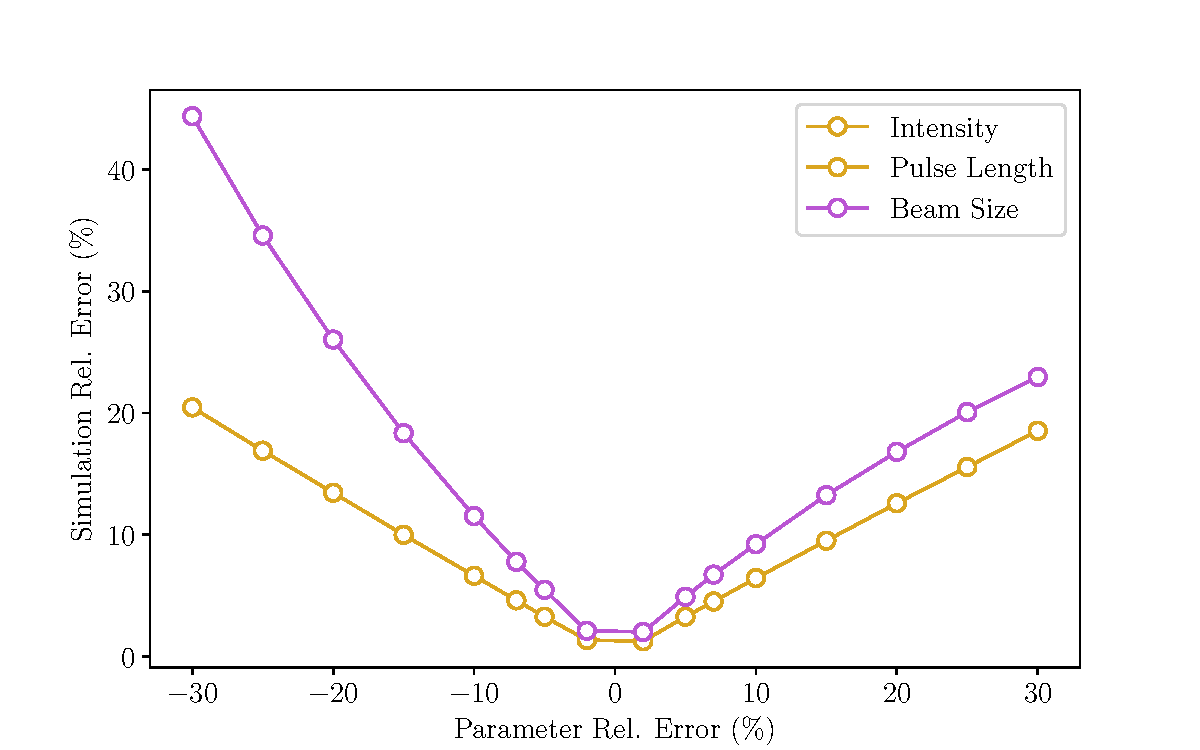
\includegraphics[width=1.0\columnwidth]{BeamParameterUncertainty/BeamParUnc.pdf}
    \caption{Effects of beam parameter uncertainties on maximum temperature simulation results.}
    \label{fig:BeamParUnc}
\end{figure}

It is difficult to give a specific value of the Beam parameters uncertainty, as it is very much dependent on the simulation case. If the range of confidence of the simulation studies is necessary for a certain application a proper study of the Beam parameter uncertainties should be carried out. 

\subsection{Material Parameter Uncertainties.}

Material parameters are all those material properties that are necessary for the simulation. These properties are compiled in Table \ref{tab:MaterialProp}. In most cases, the values of these parameters are well known and can be found in the literature. A very good reference for metallic and non-metallic properties of solids is \parencite[][]{ref:MatProperties}.  

\begin{table}[h]
    \centering
    \begin{tabular}{ccc}
    \hline
    \textbf{Property} & \textbf{Abbreviation} & \textbf{Units} \\ \hline
    Atomic Number     & Z                     &                \\
    Atopic Mass       & A                     & amu            \\
    Density           & rho                   & g/cm3          \\
    Melting Point     & Mp                    & K              \\
    Work Funktion     & phi                   & eV             \\
    Emissivity        & eps                   &                \\
    Specific Heat     & Cp                    & J/gK           \\
    Conductivity      & k                     & W/mK           \\ \hline
    \end{tabular}
    \caption{Material parameters necessary for thermal simulations.}
    \label{tab:MaterialProp}
\end{table}

Similarly to the beam parameter case, figure  \ref{fig:MatPar} shows the effects uncertainties in the different material parameters have on the final maximum temperature uncertainties. In this case, one can observe how the parameter that induces the highest uncertainty is the specific heat (Cp). How big are the uncertainties is very much dependent on the material. To give a numerical example of typical uncertainty values we studied the Graphite and the tungsten case. 
\begin{figure}[h]
    \centering
    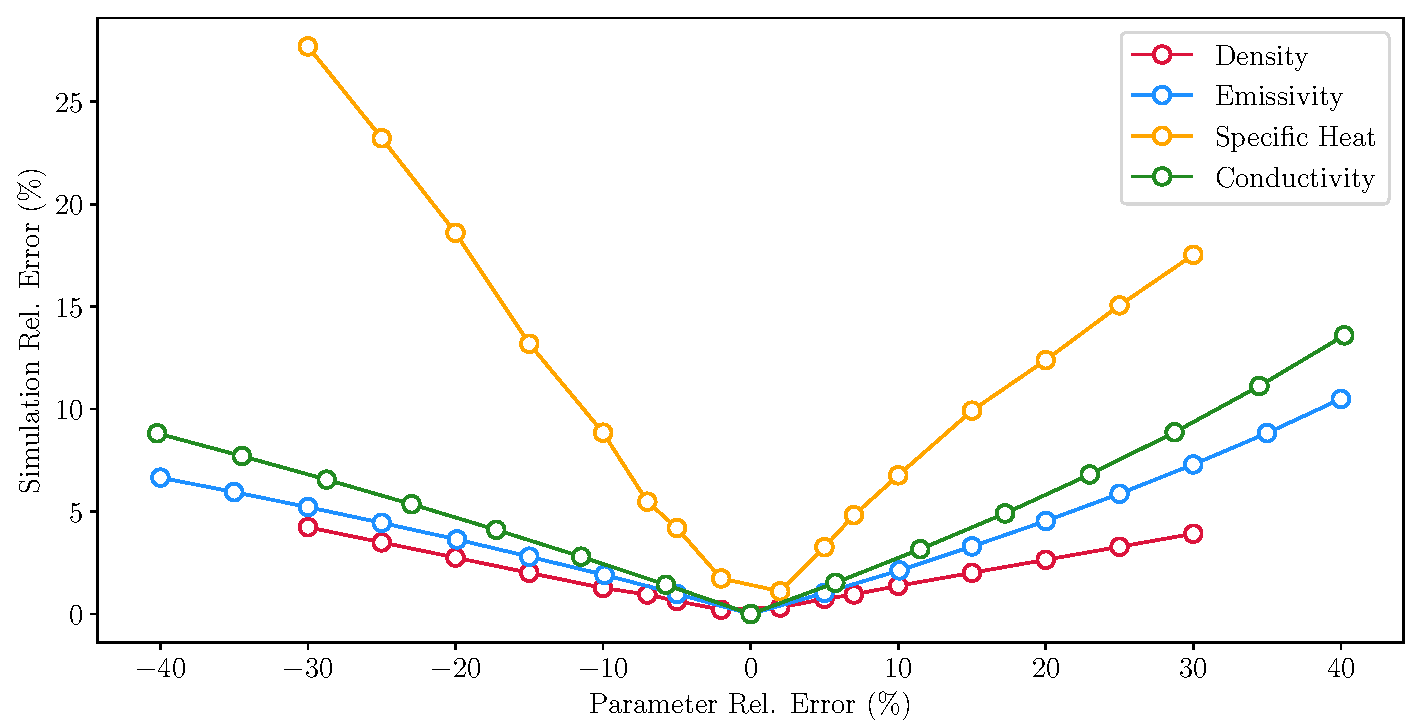
\includegraphics[width=1.0\columnwidth]{MaterialParameterUncertainty/MatParUnc.pdf}
    \caption{Effects of material property uncertainties on maximum temperature results.}
    \label{fig:MatPar}
\end{figure}

Figure \ref{fig:MatPropUnc} shows the uncertainties for specific heat, emissivity and thermal conductivity parameters for Tungsten and Graphite. In this case, the uncertainties for the other parameters were negligible. The central points on the boxes represent the average property value, while the limits of the colored boxes represent the RMS. The error bars represent the maximum and minimum discrepancies found with respect to the average value. 
\begin{figure}[h]
    \centering
    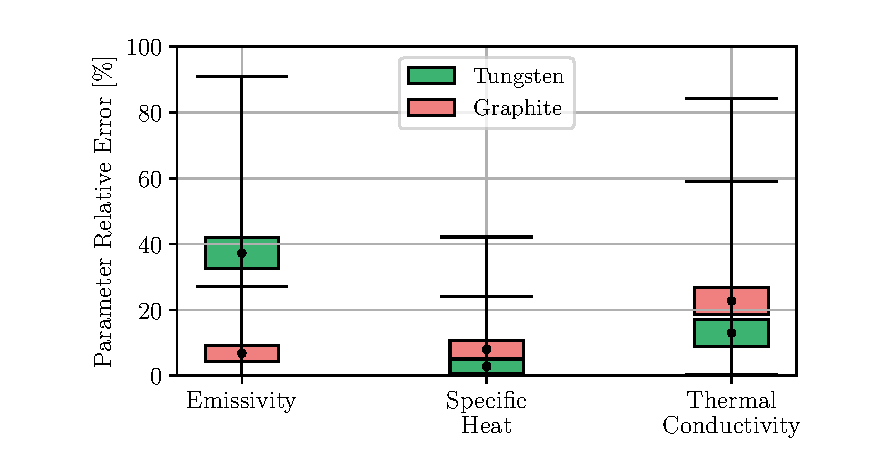
\includegraphics[width=1.0\columnwidth]{PlotTungstenGraphiteUncertainty/GraphTungsUnc.pdf}
    \caption{Material property uncertainties for Graphite and Tungsten. }
    \label{fig:MatPropUnc}
\end{figure}

Uncertainties of the Specific heat are quite small ($2.83 \% $) for both graphite and tungsten. In the case of graphite, values for the emissivity seem to be quite well known ( $ 6.75\%$). Contrarily, a much higher uncertainty was found in the case of its thermal conductivity ( $ 22.71\%$). In the case of tungsten, we find the opposite situation, different sources seem to agree on the value of the thermal conductivity ($13.0\%$ ), however, big uncertainties are found in the emissivity case ($43.26 \%$). 

This big uncertainty in the tungsten emissivity led to an in-depth investigation. To reduce the overall uncertainty of the simulations for tungsten detectors. These experimental measurements and the obtained results will be covered in Chapter \ref{ch:EmissivityMeas}.
